\documentclass[tikz]{standalone}
\usepackage{pgfplots}
\begin{document}


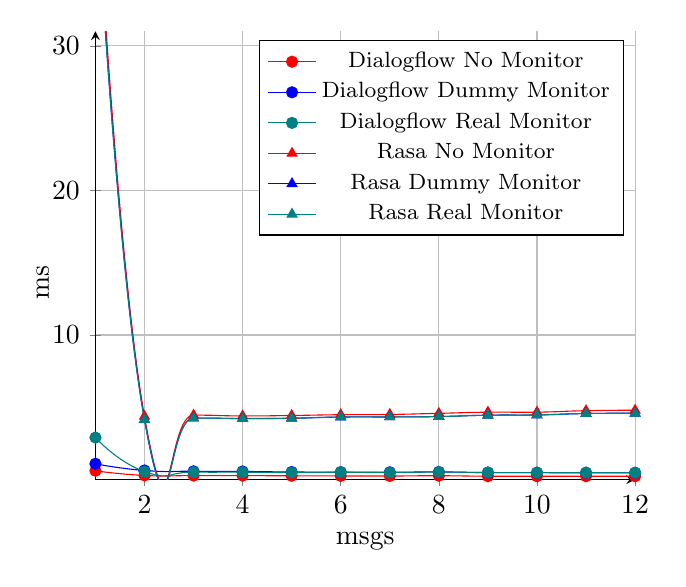
\begin{tikzpicture}
\begin{axis}[axis lines=middle, grid=both, ymin=0, ymax=31, legend style={font=\footnotesize}, xlabel=msgs, ylabel=ms,xlabel style={at={(ticklabel cs:0.5)}, anchor=north}, ylabel style={at={(ticklabel cs:0.5)}, anchor=east, rotate=90},]
\addplot [red, smooth, tension=1, mark=*] coordinates {(1, 0.615)(2, 0.292)(3, 0.28)(4, 0.278)(5, 0.268)(6, 0.258)(7, 0.253)(8, 0.27)(9, 0.238)(10, 0.237)(11, 0.237)(12, 0.234)};
\addplot [blue, smooth, tension=1, mark=*] coordinates {(1, 1.1)(2, 0.637)(3, 0.578)(4, 0.567)(5, 0.531)(6, 0.523)(7, 0.513)(8, 0.533)(9, 0.489)(10, 0.483)(11, 0.478)(12, 0.476)};
\addplot [teal, smooth, tension=1, mark=*] coordinates {(1, 2.91)(2, 0.559)(3, 0.521)(4, 0.515)(5, 0.493)(6, 0.511)(7, 0.491)(8, 0.524)(9, 0.491)(10, 0.483)(11, 0.484)(12, 0.481)};
\addplot [red, smooth, tension=1, mark=triangle*] coordinates {(1, 42.782)(2, 4.375)(3, 4.458)(4, 4.407)(5, 4.439)(6, 4.491)(7, 4.51)(8, 4.586)(9, 4.665)(10, 4.667)(11, 4.768)(12, 4.799)};
\addplot [blue, smooth, tension=1, mark=triangle*] coordinates {(1, 41.771)(2, 4.155)(3, 4.252)(4, 4.228)(5, 4.247)(6, 4.329)(7, 4.338)(8, 4.364)(9, 4.457)(10, 4.475)(11, 4.572)(12, 4.589)};
\addplot [teal, smooth, tension=1, mark=triangle*] coordinates {(1, 41.734)(2, 4.147)(3, 4.254)(4, 4.223)(5, 4.253)(6, 4.332)(7, 4.34)(8, 4.366)(9, 4.458)(10, 4.48)(11, 4.574)(12, 4.587)};
\legend{Dialogflow No Monitor, Dialogflow Dummy Monitor, Dialogflow Real Monitor, Rasa No Monitor, Rasa Dummy Monitor, Rasa Real Monitor}
\end{axis}
\end{tikzpicture}
\end{document}